\chapter{Potential Outcomes}
\label{ch-pot-out-2d}
This chapter
is based on Ref.\cite{book-mixtape},
a book by Stephen Cunningham entitled
``Causal inference: the mixtape".

The theory of potential
outcomes (PO) was for the most part
invented in a seminal
1974 paper by Donald B. Rubin. Rubin
has also
made important extensions
to PO theory since 1974. However, he refuses to
use Pearl's causal DAGs to discuss PO theory.
Pearl has shown that PO theory
can be substantially clarified
and extended by using
the language of causal DAGs.
The d-separation theorem
that we discuss in  Chapter \ref{ch-dsep}
is especially
useful in this regard.


In this chapter, we stress the
connection
of PO theory to bnets,
and, in particular, to
the do and imagine operators
defined in Chapter \ref{ch-counterf}. Hence,
before reading this chapter,
the reader is expected to have at least
skimmed  Chapter \ref{ch-counterf},
so that he/she understands
the definition
of do and imagine operators.

\begin{table}[h!]
\centering
\begin{tabular}{|l|l|l|l|l|}
\hline
\rowcolor[HTML]{ECF4FF}
$\s$ & $\rvd^\s$ & $\rvy^\s$ & $\rvy^\s(0)$ & $\rvy^\s(1)$ \\ \hline
Edith & 0 & 5 & 5 & . \\ \hline
Frank & 0 & 7 & 7 & . \\ \hline
George & 0 & 8 & 8 & . \\ \hline
Hank & 0 & 10 & 10 & . \\ \hline
Andy & \cellcolor[HTML]{FFFFC7}1 & 10 & . & 10 \\ \hline
Ben & \cellcolor[HTML]{FFFFC7}1 & 5 & . & 5 \\ \hline
Chad & \cellcolor[HTML]{FFFFC7}1 & 16 & . & 16 \\ \hline
Daniel & \cellcolor[HTML]{FFFFC7}1 & 3 & . & 3 \\ \hline
\end{tabular}
\caption{PO dataset describing whether
individual $\s$
took a treatment dose ($d^\s=1$)
or didn't ($d^\s=0$).
The
treatment outcome
is measured by the real number $y^\s$.}
\label{tab-pot-out-missing}
\end{table}

Suppose a {\bf population
of individuals} $\s=0,1,2, \ldots, nsam-1$
is given ($d^\s=1$) or
not given ($d^\s=0$)
a {\bf treatment discrete drug dose} $d^\s$,
and that
the
 {\bf treatment outcome (i.e., response)}
is measured by
a real number $y^\s$.
Table \ref{tab-pot-out-missing}
gives a possible {\bf PO dataset}
for this scenario.
As you
can see from
that table,
each individual
either takes a drug
dose or
doesn't,
but not both.
PO theory
can be viewed as a
 {\bf  missing
data (MD) problem}. MD problems are
discussed in
 Chapter \ref{ch-missing-d}.
However, the PO MD problem
is much more specialized
than the generic MD problems
discussed in Chapter \ref{ch-missing-d}.
In the PO MD
problem, we can
fill
in the blank cells
by matching
each individual
that took
the drug with
another {\it similar}
individual that didn't.
We will have much
more to say about
this matching
strategy later in this chapter.

One can define
similar
individuals as
individuals that have the same
value
for $nx$ features $x^\s=(x^\s_i)_{i=0, 1, \ldots, nx-1}$.
One
can add to Table \ref{tab-pot-out-missing}
 $nx$ extra columns
giving the value of
the feature vector $x^\s$
for each individual.
Members
of a population with
the same $x^\s$
are referred to as
a
{\bf subpopulation or stratum (i.e., layer)}.

In a {\bf randomized controlled trial (RCT)}
\footnote{The term {\bf A/B test}
is often used to mean a RCT
where A and B are the treated and control groups. However,
sometimes the term is used to refer to
an experiment  that conditions on confounders,
which violates the definition of a RCT,
and is the same as a PO test.},
the effect
of the variable $x^\s$ on
the value
of $d^\s$
is eliminated by
randomizing
the population
and therefore
making the effect of $x^\s$
average out  to zero.
However,
there are many situations
in which carrying out a RCT is not
possible. PO theory is
a way of predicting the
result
of a RCT in situations where
doing a real RCT is not physically possible.

In this chapter, $x^\s$
will be called the confounders.
Implicit throughout this chapter
is the assumption that there are {\bf
no unmeasured confounders}.
Because if
there are some unmeasured confounders,
those can
send secret messages
that influence the value
that $d^\s$ takes.
This would ruin
the
predictions
of someone trying
to predict the results of a RCT
without
being privy to those secret
messages.
When there are {\bf some
unmeasured confounders},
it might still be
possible
to
predict the effect of a RCT.
This might be possible
using instrumental variables. See Chapter
\ref{ch-instrumental}
for a discussion
of {\bf instrumental
variables}.


\section{$G$ and $G_{den}$,
bnets,
the starting point bnets}


\begin{figure}[h!]
$$
\begin{array}{ccc}
\xymatrix{
&\rvx\sqsig\ar[dl]\ar[dr]
\\
\rvd\sqsig\ar[rr]&&\rvy\sqsig
}
&&
\xymatrix{
u_\rvd\ar[dd]&u_\rvx\ar[d]&u_\rvy\ar[dd]
\\
&\rvx\ar[dl]\ar[dr]
\\
\rvd\ar[rr]&&\rvy
}
\\
\\
G&&G_{den}
\end{array}
$$
\caption{Bnets
$G$ and $G_{den}$
are
our starting
point in discussing PO theory.
 $G$ is for
a single individual $\s$ of the
population.
Bnet $G_{den}$ is the
DEN counterpart
to $G$.
DEN (Deterministic with
External Noise) bnets are discussed in Chapter
\ref{ch-linear-sys}.}
\label{fig-po-G-start}
\end{figure}

In this chapter, we will
abbreviate
$\rvX\sqsig=\rvX^\s$
for
$X\in \{d, x, y\}$
and for $\s=\{0,1,2, \ldots, nsam-1\}$.


For each individual (aka unit, sample)
$\s=0, 1, 2, \ldots nsam-1$, let:

$\rvd^\s\in\bool$: treatment discrete drug dose,  1 if treated and 0 if untreated

$\rvy^\s\in \RR$:
 treatment potential outcome

$\rvx^\s$: column vector of treatment
confounders
(aka covariates because they
are often used as covariates (i.e.,
independent
variables) in linear regression.)

Consider bnets $G$ and $G_{den}$
in
 Fig.\ref{fig-po-G-start}.
$G$ reflects the language
used in Ref.\cite{book-mixtape}
to discuss PO theory. And
$G_{den}$ reflects
the language that Judea Pearl
prefers to use to discuss PO theory.
Both languages are equivalent. To go from
one language to the other, one need only
perform the following
swaps, where $\rvu$
is the external noise of the DEN bnet.

$\rvX^\s\leftrightarrow \rvX(\rvu)$
for $X\in \{d, x, y\}$.

$P(\s)=\frac{1}{nsam}\leftrightarrow P(u)$

$\sum_\s P(\s) (\cdot)
\leftrightarrow \sum_uP(u) (\cdot)$




The TPMs, printed in blue,
for the bnet
$G$
in Fig.\ref{fig-po-G-start},
are as follows:


\beq\color{blue}
P(x^\s)=
P_{\rvx}(x^\s)
\eeq

\beq\color{blue}
P(d^\s|x^\s)=
P_{\rvd|\rvx}(d^\s|x^\s)
\eeq


\beq\color{blue}
P(y^\s| d^\s, x^\s)=
P_{\rvy|\rvd, \rvx}(y^\s|d^\s, x^\s)
\eeq




Now let:

$\rvd\in\bool$: treatment discrete drug dose,  1 if treated and 0 if untreated

$\rvy\in \RR$:
 treatment potential outcome

$\rvx$: column vector of
treatment
confounders (aka covariates)


$\rvu=(\rvu_\rvd, \rvu_\rvx, \rvu_\rvy)$:
external noise

The TPMs, printed in blue,
for the bnet
$G_{den}$
in Fig.\ref{fig-po-G-start},
are as follows:


\beq \color{blue}
P(x|u_\rvx)= \indi(\;\;x=u_\rvx\;\;)
\eeq

\beq\color{blue}
P(d|x, u_\rvd)=
\indi( \;\; d= f_\rvd(x, u_\rvd)
\;\;)
\eeq

\beq\color{blue}
P(y|d,x, u_\rvy)=
\indi( \;\; y= f_\rvy(d,x, u_\rvy)
\;\;)
\label{eq-y-is-fy}
\eeq

If we linearize
 $f_\rvy$ in Eq.(\ref{eq-y-is-fy}),
we get

\beqa
\rvy =
\delta \rvd + \beta \rvx + \rvu_\rvy
\;,
\label{eq-y-is-lin}
\eeqa
where $\delta, \beta\in \RR$.
Assuming
that $\rvx, \rvy\in \RR$
and $\rvd\in \bool$,
Eq.(\ref{eq-y-is-lin}) can be plotted.
The resulting plot
is given in Fig.\ref{fig-po-two-parallel-lines}.
This plot
is a very special
case of the PO problem,
but it gives a crude idea
of the ``effects" $\delta
= y(1)-y(0)$ that PO theory
gives estimates for.
Any
individual participating in the experiment
experiences either $y(1)$
or $y(0)$,
but not both.



\begin{figure}[h!]
\centering
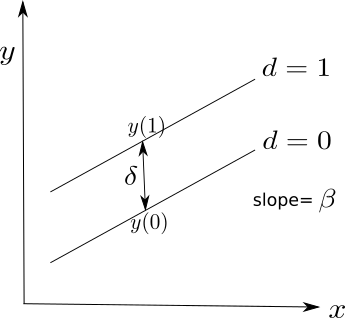
\includegraphics[width=2in]
{pot-out/two-parallel-lines.png}
\caption{Plot  of
Eq.(\ref{eq-y-is-lin})}
\label{fig-po-two-parallel-lines}
\end{figure}




\section{$G_{do+}$  bnet}
\begin{figure}[h!]
$$
\begin{array}{ccccc}
\xymatrix{
&\rvx^\s\ar[dr]\ar[dl]
\\
\rvd^\s\ar[rr]&&\rvy^\s
}
&&
\xymatrix{
&\rvx^\s\ar[dr]
\\
\cald\rvd^\s=\td^\s\ar[rr]&&\rvy^\s
}
&&
\xymatrix{
&\rvx^\s\ar[dr]
\\
\cald\rvd^\s\ar[rr]&&\rvy^\s
}
\\
\\
G&&G_{do}= \cald_{\rvd^\s}
(\td^\s)G&& G_{do+}
\end{array}
$$
\caption{Bnet $G_{do}= \cald_{\rvd^\s}
(\td^\s)G$
is obtained by applying
the do operator to node $\rvd^\s$
of bnet $G$. Bnet $ G_{do+}$
is obtained
by adding a prior
probability distribution $P(\td^\s)$
to node $\cald\rvd^\s$ of
bnet $G_{do}$.}
\label{fig-po-G-do}
\end{figure}

Fig.\ref{fig-po-G-do}
shows how bnet $G_{do}$
is obtained by applying
the do operator to bnet $G$,
and
how
bnet $G_{do+}$
is obtained by adding
a prior
probability distribution
 to one of the nodes
of $G_{do}$.
In bnet $G_{do}$,
node  $\rvd^\s$ has been
stripped of all outside
influences and fixed to a
specific state $\td^\s$.
This is what a RCT does.

The TPMs, printed in blue,
for the bnets $G_{do}$
and $G_{do+}$,
are as follows.
Note that the TPMs
for bnets  $G_{do}$ and $G_{do+}$
are defined in terms
of the TPMs of bnet $G$.

\beq\color{blue}
P(x^\s)=
P_{\rvx}(x^\s)
\eeq

\beq
P_{\cald\rvd}(\td)=\sum_x P_{\rvd|\rvx}
(\td|x)P_\rvx(x)
\eeq

\beq\color{blue}
P(\td^\s)=
\left\{
\begin{array}{ll}
\delta(\td^\s, (\td^\s)')& \text{for $G_{do}$}
\\
P_{\cald\rvd}(\td^\s)
& \text{for $G_{do+}$}
\end{array}
\right.
\eeq

\beq\color{blue}
P(y^\s|\td^\s, x^\s)=
P_{\rvy|\rvd, \rvx}(y^\s|\td^\s, x^\s)
\eeq




\section{$G_{im+}$ bnet}


\begin{figure}[h!]
$$
\begin{array}{ccccc}
\xymatrix{
&\rvx^\s\ar[dl]\ar[dr]
\\
\rvd^\s\ar[rr]&&\rvy^\s
}
&&
\xymatrix{
&\rvx^\s\ar[dl]\ar[dr]
\\
\rvd^\s&\rvtd^\s=\td^\s\ar[r]&\rvy^\s
}
&&
\xymatrix{
&\rvx^\s\ar[dl]\ar[dr]
\\
\rvd^\s&\rvtd^\s\ar[r]&\rvy^\s
}
\\
\\
G&&G_{im}= \cali_{\rvd^\s\rarrow\rvy^\s}
(\td^\s)G&&G_{im+}
\end{array}
$$
\caption{Bnet
$G_{im}= \cali_{\rvd^\s\rarrow\rvy^\s}
(\td^\s)G$
is obtained by applying
the imagine operator to arrow
$\rvd^\s\rarrow\rvy^\s$
of bnet $G$. Bnet $ G_{im+}$
is obtained
by adding a prior
probability distribution $P(\td^\s)$
to node $\rvtd^\s$ of
bnet $G_{im}$.
}
\label{fig-po-G-im}
\end{figure}

Fig.\ref{fig-po-G-im}
shows how bnet $G_{im}$
is obtained by applying
an imagine operator to bnet $G$,
and how bnet $G_{im+}$
is obtained  by adding
a prior
probability distribution to
one of the nodes of $G_{im}$.
$\rvd\in \bool$ represents the
dose that a patient
is told to take by a doctor, and
$\rvtd\in \bool$ represents the
dose he actually takes.
If $\rvd=\rvtd$, the
patient is compliant,
and if $\rvd\neq\rvtd$, he is
non-compliant.


The TPMs, printed in blue,
for the nodes of bnets $G_{im}$ and $G_{im+}$,
are as follows.
Note that the TPMs
for bnets  $G_{im}$ and $G_{im+}$
are defined in terms
of the TPMs of bnet $G$.
Note that
the prior
$P(\td)$ is not arbitrary;
it's calculated from
the TPMs of bnet $G$.


\beq\color{blue}
P(x^\s)=
P_{\rvx}(x^\s)
\eeq

\beq\color{blue}
P(d^\s|x^\s)=
P_{\rvd|\rvx}(d^\s|x^\s)
\eeq

\beq
\pi_\td=P(\td)=\sum_x P_{\rvd|\rvx}
(\td|x)P_\rvx(x)
\eeq

\beq\color{blue}
P(\td^\s)=
\left\{
\begin{array}{ll}
\delta(\td^\s, (\td^\s)')& \text{for $G_{im}$}
\\
\pi_{\td^\s}
& \text{for $G_{im+}$}
\end{array}
\right.
\eeq


\beq\color{blue}
P(y^\s|\td^\s, x^\s)=
P_{\rvy|\rvd, \rvx}(y^\s|\td^\s, x^\s)
\eeq



\section{$G_{im+}$ bnet
with nodes $y^\sigma(0),
y^\sigma(1)$ added to it.}


\begin{figure}[h!]
$$
\begin{array}{ccccc}
\xymatrix{
&\rvx^\s\ar[ddl]\ar[ddr]
\\
\\
\rvd^\s\ar[rr]&&\rvy^\s
}
&
\xymatrix{
&\rvx^\s\ar[ddl]\ar[dr]
\\
&&[\rvy^\s(0),\rvy^\s(1)]\ar[d]
\\
\rvd^\s&\rvtd^\s=\td^\s\ar[r]
\ar[ur]&\rvy^\s
}
&
\xymatrix{
&\rvx^\s\ar[ddl]\ar[dr]
\\
&&[\rvy^\s(0),\rvy^\s(1)]\ar[d]
\\
\rvd^\s&\rvtd^\s\ar[r]\ar[ur]
&\rvy^\s
}
\\
G&G_{im}= \cali_{\rvd^\s\rarrow\rvy^\s}
(\td^\s)G&G_{im+}
\end{array}
$$
\caption{
Fig.\ref{fig-po-G-im}
with two new nodes $\rvy^\s(0)$
and $\rvy^\s(1)$ added to bnets $G_{im}$
and $G_{im+}$.
The tuple node $[\rvy^\s(0), \rvy^\s(1)]$
can also be represented by
two nodes $\rvc\rarrow\rvy(\rvc)$,
where $\rvc\in \bool$.
}
\label{fig-po-G-im-y0-y1}
\end{figure}



Consider Fig.\ref{fig-po-G-im-y0-y1},
which was obtained by adding two new
nodes $\rvy^\s(0)$
and $\rvy^\s(1)$
to bnets $G_{im}$
and $G_{im+}$ in
Fig.\ref{fig-po-G-im}.
The
TPMs, printed in blue,
 for bnets $G_{im}$ and $G_{im+}$,
are as follows. Note
that we define them in terms
of the TPMs
for bnet $G$.

\beq\color{blue}
P(x^\s)=
P_{\rvx}(x^\s)
\eeq

\beq\color{blue}
P(d^\s|x^\s)=
P_{\rvd|\rvx}(d^\s|x^\s)
\eeq

\beq
\pi_\td=P(\td)=\sum_x P_{\rvd|\rvx}
(\td|x)P_\rvx(x)
\eeq

\beq\color{blue}
P(\td^\s)=
\left\{
\begin{array}{ll}
\delta(\td^\s, (\td^\s)')& \text{for $G_{im}$}
\\
\pi_{\td^\s}
& \text{for $G_{im+}$}
\end{array}
\right.
\eeq


\beq\color{blue}
P(y^\s(0)|\td^\s, x^\s) =
P_{\rvy(0)|\rvtd, \rvx}(y^\s(0)|\td^\s, x^\s)
\eeq

\beq\color{blue}
P(y^\s(1)|\td^\s, x^\s) =
P_{\rvy(1)|\rvtd, \rvx}(y^\s(1)|\td^\s, x^\s)
\eeq


\beqa\color{blue}
P(y^\s|y^\s(0), y^\s(1), \td^\s)=
&=&\color{blue}
\indi(y^\s= \td^\s y^\s(1) + (1-\td^\s)y^\s(0))
\\
&=&\color{blue}
\indi(y^\s= y^\s(\td^\s))
\label{eq-y-equal-ytd}
\eeqa

If we sum over the
nodes $\rvy(0)$ and $\rvy(1)$
of this bnet, we should
get the bnet $G_{im}$
of Fig.\ref{fig-po-G-im} that
we discussed previously,
which is the same as this
bnet but without the nodes
$\rvy(0)$ and $\rvy(1)$.
This is easy to check. Indeed,

\begin{align}
P(y^\s|\td^\s, x^\s)
&=
\sum_{y^\s(0)}
\sum_{y^\s(1)}
\indi(y^\s= y^\s(\td^\s))
P(y^\s(0)|\td^\s, x^\s)
P(y^\s(1)|\td^\s, x^\s)
\\
&=
\left\{
\begin{array}{ll}
P_{\rvy(0)|\rvtd, \rvx}(
y^\s|\td^\s, x^\s)&\text{ if }
\td^\s=0
\\
P_{\rvy(1)|\rvtd, \rvx}(
y^\s|\td^\s, x^\s)&\text{ if }
\td^\s=1
\end{array}
\right.
\;.
\label{eq-y-is-y-td}
\end{align}
\begin{mdframed}[hidealllines=true,backgroundcolor=gray!10]
Note that
$P(\rvy(c)=y|\rvtd=\td, x)$
for $c, \td\in \bool$
are four
different probability
distributions,
and that
$P(\rvy=y|\td=\td,x)$
is defined in terms
of two of them, the
so called {\bf factual
distributions} with $c=\td$.
By measuring $\rvy$,
we can't access the other
2 probability distributions,
the so called {\bf counterfactual
distributions}
with $c\neq\td$.
\end{mdframed}

\section{Expected Values of
 treatment outcome $y^\sigma$}

It is convenient
to define
the following
expected values of
$\rvy^\s$
in terms of the TPMs of
bnet $G_{im+}$:

\beq
\calr_{c|d,x}
=
E_{\s|d,x}[\rvy^\s(c)]
\rarrow
E_{\rvy|d,x} [\rvy(c)]
=\sum_{y} y
P(\rvy(c)=y|\rvd=d,x)
\eeq

\beq
\caly_{c|\td,x}
=
E_{\s|\td,x}[\rvy^\s(c)]
\rarrow
E_{\rvy|\td,x} [\rvy(c)]
=\sum_{y} y
P(\rvy(c)=y|\rvtd=\td,x)
\label{eq-need-positivity}
\eeq

\beq
\caly_{c|\td}
=
E_{\s| \td}[\rvy^\s(c)]
\rarrow
E_{\rvy|\td} [\rvy(c)]
=\sum_x \caly_{c|\td,x}
\underbrace{P(x|\td)}_
{=P(x)\text{ by d-separation}}
\eeq


\beq
\caly_{c|x}
=
E_{\s| x}[\rvy^\s(c)]
\rarrow
E_{\rvy|x} [\rvy(c)]
=\sum_\td \caly_{c|\td,x}
\underbrace{P(\td|x)}_
{=P(\td) \text{ by d-separation}}
\eeq

\beq
\caly_{c}
=
E_{\s}[\rvy^\s(c)]
\rarrow
E_{\rvy} [\rvy(c)]
=\sum_{\td,x}\caly_{c|\td,x}
 P(\td)P(x)
\eeq

Also let

\beq
\caly_{|\td,x}
=
E_{\s| \td, x}[\rvy^\s]
\rarrow
E_{\rvy|\td, x} [\rvy]
=\sum_y y P(\rvy=y|\rvtd=\td, x)
\eeq


$\caly_{|\td}, \caly_{|x}, \caly$ are 
defined analogously from 
$\caly_{|\td, x}$.

$\caly_{0|0}, \caly_{1|1}$
are said to be {\bf factual}
(indicating compliant patients)
whereas
$\caly_{0|1}, \caly_{1|0}$
are said to be {\bf counterfactual}
(indicating non-compliant patients).


\section{Translation Dictionary}

{\renewcommand{\arraystretch}{1.5}
\begin{table}[h!]
\centering
\begin{tabular}{|l|l|}
\hline
\rowcolor[HTML]{ECF4FF}
In standard PO notation&
In our notation
(for $G_{im}$ or  $G_{im+}$)\\
\hline
$i$, individual (i.e., unit, sample) index& $\s$ \\
\hline
$D_i=d_i$, treatment dose & $\rvd^\s=d^\s$\\
\hline
$Y_i=y_i$, treatment outcome& $\rvy^\s=y^\s$ \\
\hline
$X_i=x_i$, treatment confounders& $\rvx^\s=x^\s$ \\
\hline
$E[Y_i(c)]$ &
$E_{\s}[\rvy^\s(c)]=\caly_{c}$ \\
\hline
$E[Y_i|D_i=\td]$ &
$ E_{\s|\td}[\rvy^\s]=\caly_{|\td}$\\
\hline
$E[Y_i(c)|D_i=\td]$ &
$E_{\s|\td}[\rvy^\s(c)]=\caly_{c|\td}$\\
\hline
$E[Y_i(c)|D_i=\td, X_i=x]$ &
$E_{\s|\td,x}[\rvy^\s(c)]=\caly_{c|\td,x}$\\
\hline
\end{tabular}
\caption{Dictionary for
translating
from standard PO notation
of Ref.\cite{book-mixtape} to our notation.
}
\label{tab-pot-out-dict}
\end{table}
}

Table \ref{tab-pot-out-dict}
gives a dictionary for
translating
from the standard PO notation
of Ref.\cite{book-mixtape}
to our notation. $c,\td\in \bool$.
I find
 the standard PO notation
confusing because it often uses $D_i$
to represent two different nodes,
$\rvd^\s$ and $\rvtd^\s$ in $G_{im+}$.

\section{${\cal Y}_{|\tilde{d},x}
={\cal Y}_{\tilde{d}|\tilde{d},x}$}


\begin{claim}\footnote{In the
standard PO notation,
this is the frequently used identity
$$E[Y|D=d, x]= E[Y(d)|D=d, x]$$.}\label{cl-caly-bardx}
\beq
\caly_{|\td, x}=\caly_{\td|\td,x}
\eeq
\end{claim}
\proof

\beqa
\caly_{|\td,x}
&=&
\sum_y y P(\underbrace{\rvy}_
{=\rvy(\td)
\text{ by Eq.(\ref{eq-y-equal-ytd})}}
=y|\td, x)
\\
&=&
\caly_{\td|\td, x}
\;.
\eeqa
\qed



\section{Conditional Independence Assumption (CIA)}

The {\bf Conditional Independence Assumption}
 (CIA)
is said to hold
 if
\beq
(\rvy^\s(0), \rvy^\s(1),
\rvy^\s,\rvtd^\s)\perp_P\rvd^\s | \rvx^\s
\;.
\label{eq-CIA2}
\eeq
This is satisfied by $G_{im}$. To
prove this, check that

\beq
(\rvy^\s(0),\rvy^\s(1),
\rvy^\s,\rvtd^\s)
\perp_{G_{im}} \rvd^\s|\rvx^\s
\;
\eeq
and then invoke
the d-separation theorem
(see Chapter \ref{ch-dsep}).

Note that
by swapping $\rvd^\s$ and
$\rvtd^\s$ in Eq.(\ref{eq-CIA2})
we get false statements:

\beq
(\rvy^\s(0),\rvy^\s(1))
\perp_{G_{im}} \rvtd^\s|\rvx^\s
\;\;
\text{ is FALSE.}
\eeq

\beq
(\rvy^\s(0),\rvy^\s(1))
\perp_{G_{im}} \rvtd^\s
\;\;
\text{ is FALSE.}
\eeq

\beq
\rvy^\s\perp_{G_{im}} \rvtd^\s|\rvx^\s
\;\;
\text{ is FALSE.}
\eeq


A {\bf Randomized Control Trial (RCT)}
is defined to satisfy
Eq.(\ref{eq-CIA2}) without the
 $\rvx^\s$ conditioning; i.e., it
satisfies

\beq
(\rvy^\s(0), \rvy^\s(1),
\rvy^\s,\rvtd^\s)\perp_P\rvd^\s
\;.
\label{eq-CIA-minus-x}
\eeq
This means that in a RCT,
the arrow from
$\rvx^\s$ to  $\rvd^\s$ in $G_{im}$
has a vanishingly small
conditional  probability.

Because of CIA,

\begin{subequations}
\beq
\underbrace{E_{\s|\td,x}[\rvy^\s(c)]}_{\caly_{c|\td,x}}
=
E_{\s}[\rvy^\s(c)|\rvtd^\s=\td, \rvx^\s=x]
{\;\;\color{red}\neq\;\;}
E_{\s}[\rvy^\s(c)|\rvx^\s=x]=
\underbrace{E_{\s|x}[\rvy^\s(c)]}_{\caly_{c|x}}
\;,
\eeq
but

\beq
\underbrace{E_{\s|d,x}[\rvy^\s(c)]}_
{\calr_{c|d,x}}
=
E_{\s}[\rvy^\s(c)|\rvd^\s=d, \rvx^\s=x]
{\;\;\color{red}=\;\;}
E_{\s}[\rvy^\s(c)|\rvx^\s=x]
=
\underbrace{E_{\s|x}[\rvy^\s(c)]}_{\caly_{c|x}}
\;,
\label{eq-pseudo-rct}
\eeq

\label{eq-d-td-diff}
\end{subequations}

In a RCT, Eqs.(\ref{eq-d-td-diff})
are valid without the $x$ conditioning.



$E_{\s|\td,x}[\rvy^\s(c)]$
is mentioned frequently because
it equals
$\caly_{c|\td,x}$
and
treatment effects are defined as a difference of two
$\caly_{c|\td,x}$.
$E_{\s|d,x}[\rvy^\s(c)]$ is seldom mentioned
because it equals $E_{\s|x}[\rvy^\s(c)]=\caly_{c|x}$.

A common mistake
arising from
not distinguishing
between $\rvd$ and $\rvtd$,
is to say that CIA implies

\beq
\caly_{c|\td,x}=\caly_{c|x}
\text{ (FALSE)}
\;,
\eeq
when what is {\it really} meant
is that CIA implies

\beq
\calr_{c|d,x}=\caly_{c|x}
\;.
\label{eq-c-bar-d-x}
\eeq



\section{Treatment Effects}

\begin{figure}[h!]
\centering
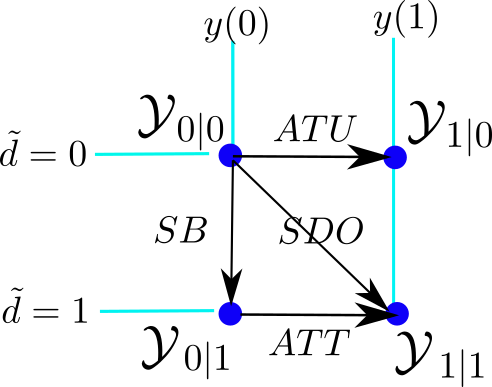
\includegraphics[width=2in]
{pot-out/y-diffs-square.png}
\caption{Different treatment effects.
A treatment effect is a difference of
two $\caly_{c|\td }$.}
\label{fig-y-diffs-square}
\end{figure}

A {\bf treatment effect} is a
a difference of two  $\caly_{c|\td }$.
It is convenient to
define the following
treatment effects.
See Fig.\ref{fig-y-diffs-square}.
In that figure, $y(c)$ appears  with
$c=0,1$.
My personal mnemonics
for $c$ and $\td$ are:
\begin{itemize}
\item
$c=1$ means being
a {\bf candidate} for treatment (i.e.,
being assigned the treatment),
and $c=0$ means not being a
candidate.
\item
$\td=1$ means being
a  {\bf doer} of the
treatment (i.e.,
complying with it)
and $\td=0$
means not being a doer.
\end{itemize}



\begin{itemize}


\item average treatment effect
 (ATE).
\beq
{\color{red}ATE}=
\caly_{1}-
\caly_{0}= \delta
\eeq
ATE= difference in
response between candidates
and non-candidates.

\item average treatment effect
of the treated (ATT)
\beq
{\color{red}ATT}=
\caly_{1|1}-\caly_{0|1}
\eeq

ATT= difference in
response between candidates
and non-candidates in doer
population.

\item average
treatment effect of the untreated (ATU)
\beq
{\color{red}ATU}=
\caly_{1|0}-\caly_{0|0}
\eeq

ATU= difference in
response between candidates
and non-candidates in non-doer
population.

\item selection bias (SB)
\beq
{\color{red}SB}=\caly_{0|1}-\caly_{0|0}
\eeq

SB= difference in response
between the doers and non-doers
in the non-candidate population.

\item simple difference in outcomes (SDO)
\beq
{\color{red} SDO}= \caly_{1|1}-\caly_{0|0}
\eeq

SDO= difference in
response between the candidate doers
and the non-candidate non-doers.

\item average
causal effect
 (ACE), used when doing a RCT.

\beq
{\color{red}ACE}=ATE \text{\;\;\;(see Claim
\ref{cl-ace-ate})}
\eeq


\end{itemize}

Note that some
of these treatment effects  are
linearly related



\beq
\underbrace{\caly_1-\caly_0}_
{ATE}=
 \underbrace{(\caly_{1|1}-\caly_{0|1})}_{ATT}\pi_1+
 \underbrace{(\caly_{1|0}-\caly_{0|0})}_{ATU}\pi_0
\label{eq-ate-att-atu}
\eeq

\beq
\underbrace{\caly_{1|1}-\caly_{0|0}}_{SDO}
=
\underbrace{(\caly_{1|1}-\caly_{0|1})}_{ATT}
+
\underbrace{\caly_{0|1}-\caly_{0|0}}_{SB}
\eeq

\beqa
\underbrace{\caly_{1|1}-\caly_{0|0}}_{SDO}
&=&
\underbrace{(\caly_{1|1}-\caly_{0|1})\pi_1 +
(\caly_{1|0}-\caly_{0|0})\pi_0 }_{ATE} \nonumber
\\
&&+
\underbrace{\caly_{0|1}-\caly_{0|0}}_{SB}\nonumber
\\
&&+
\underbrace{(\caly_{1|1}-\caly_{0|1})}_{ATT}\pi_0\nonumber
\\
&&-
\underbrace{(\caly_{1|0}-\caly_{0|0})}_{ATU}\pi_0
\label{eq-sdo-ate-else}
\eeqa

By virtue of  Eq.(\ref{eq-ate-att-atu}),

\beq
ATT=ATU\implies ATT=ATU=ATE
\;
\eeq
and

\beq
ATE=0 \iff \frac{ATU}{ATT}=-\left(\frac{\pi_1}{\pi_0}\right)
\;.
\eeq
$ATT=ATU$ ({\bf T-U symmetry}) means the
difference in
response between candidate
and non-candidate populations is
the same among
the doer and
non-doer populations.


In general, $SDO=ATT+SB$, but if there is
T-U symmetry (i.e., $ATT=ATU$),
then $SDO=ATE+SB$.

If there is T-U symmetry (i.e., $ATT=ATU$) and
zero bias (i.e., $SB=0$),
then $SDO=ATE=ATT=ATU$.

If there is a
null result
for a RCT (i.e., $ACE=ATE=0$),
T-U symmetry (i.e., $ATT=ATU$)
and zero bias (i.e., $SB=0$),
then
$SDO=ATE=ATT=ATU=0$.


Let $\cale \in\{ATE,ATT,ATU,SDO, SB\}$.
$\cale$ can be
defined for a fixed stratum $x$
by replacing $\caly_{c|\td }$
with  $\caly_{c|\td , x}$.
We will denote this restricted
version of $\cale$ by $\cale_x$.
We can calculate estimators $\hat{\cale}$
for $\cale$ using

\beq
\hat{\cale}=E_x[\hat{\cale}_x]=
\sum_x \frac{N_x}{N} \hat{\cale}_x
\;,
\eeq
where $N=nsam=\sum_x N_x$ is the
size of the population
of individuals $\s$.


ATE$_x$ is called
the {\bf Conditional
Average Treatment Effect (CATE)}.\footnote{Careful:
We define
$
ATE_x= ATT_x P_{\rvd|\rvx}(1|x) +
ATU_x P_{\rvd|\rvx}(0|x)
$. Therefore,
$
ATE_x\neq ATT_x P_{\rvd}(1) +
ATU_x P_{\rvd}(0)
$.
}





\section{Insights into
what makes treatment effects equal and
$\caly_{\tilde{d}|d}=\caly_{\tilde{d}}$}
\label{sec-td-ignored}

\begin{figure}[h!]
\centering
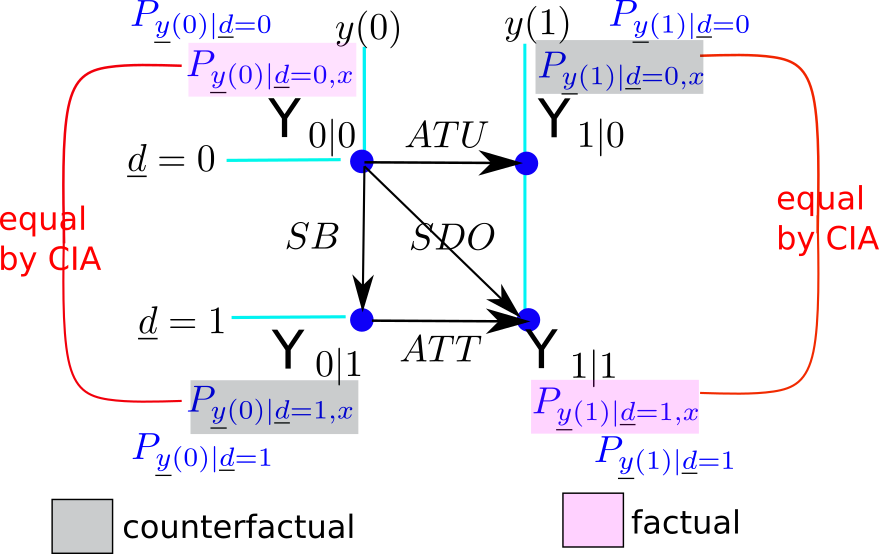
\includegraphics[width=2.5in]
{pot-out/y-diffs-square-probs.png}
\caption{Figure \ref{fig-y-diffs-square}
with added information
about  probability distributions
used to obtain each expected value
 $\caly_{c|\td }$.}
\label{fig-y-diffs-square-probs}
\end{figure}


\begin{enumerate}
\item
Is it
possible for $SDO=0$ but $ATE\neq 0$
or vice versa, and
what is going on when this is true?
\item
What is going on when two treatment effects
are equal; for instance, when $ATT=ATU$?
\item
When is $\caly_{1|0}=\caly_{1}$,
and what is going on when this is  true?
\end{enumerate}
Fig.\ref{fig-y-diffs-square-probs}
gives some
intuition
about what is
going on when any of these
things happen.

Recall that
each expected value $\caly$ has a probability
distribution $P$.
\beq
\caly_{c|\td }=\sum_{y} y P_{\rvy(c)|\rvtd}(y|\td)
\eeq
for $c, \td\in \bool$.
Fig.\ref{fig-y-diffs-square-probs}
reminds us of which $P$
is used to generate each $\caly$.
From this figure, we see that

\begin{enumerate}
\item
A sufficient
condition for $SDO=0$
is that
$P_{\rvy(1)|\rvtd=1}
=
P_{\rvy(0)|\rvtd=0}$.

\item
A sufficient condition for
$ATT=ATU$
is that
$P_{\rvy(1)|\rvtd=0}
-
P_{\rvy(0)|\rvtd=0}$
equals
$P_{\rvy(1)|\rvtd=1}
-
P_{\rvy(0)|\rvtd=1}$.
\item
A sufficient condition for $\caly_{1|0}=\caly_{1}$
is that
$P_{\rvy(1)|\rvtd=0}=
P_{\rvy(1)}$.
\end{enumerate}
$SDO=0$
depends on two corners
of the square
whereas  $\caly_{1|0}=\caly_{1}$
depends on just one corner.

\section{ACE=ATE}

Note that in $G_{do}$,

\beq
P(\rvy=y|\cald \rvd=d, \rvx=x)=
P(y|\rvd=d,x)
\;
\label{eq-rho-begone}
\eeq
because, by the d-separation
theorem,  when we condition on
the confounder $\rvx$,
we  block information from being
transmitted from $\rvd$ to $\rvy$ through $\rvx$,
and this is equivalent to
amputating the arrow $\rvx\rarrow\rvd$.

Define $ACE$ by

\begin{align}
ACE&=\sum_y y
[P(y|\cald\rvd=1)-P(y|\cald\rvd=0)]
\\
&=
\sum_x P(x)\sum_y y [P(y|\cald\rvd=1,x)-P(y|\cald\rvd=0,x)]
\\
&=
\sum_x P(x)\sum_y y [P(y|\rvd=1,x)-P(y|\rvd=0,x)]
\;. \text{ (by Eq.(\ref{eq-rho-begone}))}
\label{eq-my-backdoor-proof}
\end{align}
Eq.(\ref{eq-my-backdoor-proof} )
also follows from the backdoor criterion.


\begin{claim}\label{cl-ace-ate}
\beq
ACE=ATE
\eeq
\end{claim}
\proof

Eqs.(\ref{eq-rho-begone})
and (\ref{eq-my-backdoor-proof})
are only valid for $G_{do}$.
For $G_{im}$,
$P(\rvy=y|\cald \rvd=d, x)$
must be replaced by\footnote{
One way to rationalize this is to say
that for $G_{im}$,
in the definition of ACE,
one must not only amputate
the arrow $\rvx\rarrow \rvd$,
but
one
set both of the nodes $\rvd$ and $\rvtd$ to $d$.}
$P(\rvy(d)=d|\rvd=d,x)$
so Eq.(\ref{eq-my-backdoor-proof})
for ACE becomes


\begin{align}
ACE&=
\sum_x P(x)\sum_y y [P(\rvy(1)=y|\rvd=1,x)-
P(\rvy(0)=y|\rvd=0,x)]
\\
&=\sum_x P(x)[\calr_{1|1, x}-\calr_{0|0, x}]
\\
&=
\sum_x P(x)[\caly_{1|x}-\caly_{0|x}]
\\
&=
\caly_{1}-\caly_{0}
\\
&=
ATE
\end{align}

Note that if keep
Eq.(\ref{eq-my-backdoor-proof}) intact,
we get an unacceptable answer

\begin{align}
ACE&=
\sum_x P(x)\sum_y y [P(\rvy=y|\rvd=1,x)-P(\rvy=y|\rvd=0,x)]
\\
&=
\sum_x P(x)\sum_y y [P(\rvy=y|x)-P(\rvy=y|x)]
\\
&=0
\;,
\end{align}
and if we replace
$P(y|\rvd=d,x)$ by $P(y|\rvtd=d,x)$
in  Eq.(\ref{eq-my-backdoor-proof}),
we get another unacceptable answer
\begin{align}
ACE&=
\sum_x P(x)\sum_y y [P(\rvy=y|\rvtd=1,x)-P(\rvy=y|\rvtd=0,x)]
\\
&=
\sum_x P(x)[P(\rvy(1)=y|\rvtd=1,x)
-P(\rvy(0)=y|\rvtd=0,x)]
\\
&=
\sum_x P(x)[\caly_{1|1,x}-\caly_{0|0,x}]
\\
&=
SDO
\;.
\end{align}
\qed

We will say there is a {\bf null result
in a RCT} when $ACE=0$. By the previous claim,
this is true iff $ATE=0$.

\section{$(SDO,ATE)$ space}
If we substitute
$y^\s\rarrow y^\s(\td^\s)$ and
 $y^{m(\s)}\rarrow y^\s(!\td^\s)$,
where $!0=1$ and $!1=0$,
into
the estimator
Eq.(\ref{eq-est-ate}) for $ATE$
and the estimator
Eq.(\ref{eq-est-sdo}) for $SDO$,
we get

\beqa
\widehat{ATE}_x
&=&
\frac{1}{N_x}\sum_{\s\in A_x}
 (2\td^\s-1)[y^\s(\td^\s) -y^\s(!\td^\s)]
\\
&=&
\frac{1}{N_x}\sum_{\s\in A_x}
 [y^\s(1) -y^\s(0)]
\label{eq-est-ate-simple}
\eeqa
and

\beqa
\widehat{SDO}_x
&=&
\frac{1}{N_{1,x}}
\sum_{\s\in A_x} \td^\s y^\s(\td^\s)
-
\frac{1}{N_{0,x}}
\sum_{\s\in A_x} (1-\td^\s) y^\s(\td^\s)
\\
&=&
\frac{1}{N_{1,x}}
\sum_{\s\in A_{1,x}} y^\s(1)
-
\frac{1}{N_{0,x}}
\sum_{\s\in A_{0,x}}  y^\s(0)
\;.
\label{eq-est-sdo-simple}
\eeqa

Recall that
$\hat{\cale}=E_x[\hat{\cale}_x]=
\sum_x \frac{N_x}{N}\hat{\cale}_x$
for $\cale\in\{ATE, SDO\}$.

Recall also that
$ACE=ATE=0$ is the null
result in a RCT.


Suppose that
the treatment outcome $y^\s$
has only two
possible values, 0 and 1.
Then, $-1\leq ATE \leq 1$
and
$-1\leq SDO \leq 1$.
But does  $ATE=0$
imply $SDO=0$
or vice versa?
Next, we answer
that question
and more
by finding
the region
of accessibility in the
$(SDO, ATE)$
plane,
assuming $y^\s\in \bool$.


\newpage

\begin{figure}[h!]
\centering
\subfloat[$ATE=-1$ $(SDO=-1)$ point A]{
\begin{tabular}{|
>{\columncolor[HTML]{ECF4FF}}l |l|l|l|}
\hline
\cellcolor[HTML]{CBCEFB}$\s$ & \cellcolor[HTML]{CBCEFB}$\td^\s$ & \cellcolor[HTML]{CBCEFB}$y^\s(0)$ & \cellcolor[HTML]{CBCEFB}$y^\s(1)$ \\ \hline
1 & 0 & 1 & 0 \\ \hline
2 & 0 & 1 & 0 \\ \hline
3 & 0 & 1 & 0 \\ \hline
4 & 1 & 1 & 0 \\ \hline
5 & 1 & 1 & 0 \\ \hline
6 & 1 & 1 & 0 \\ \hline
\end{tabular}
}
\quad
\subfloat[$ATE=\frac{1}{2}$ $(SDO=0)$ point B]{
\begin{tabular}{|
>{\columncolor[HTML]{ECF4FF}}l |l|l|l|}
\hline
\cellcolor[HTML]{CBCEFB}$\s$ & \cellcolor[HTML]{CBCEFB}$\td^\s$ & \cellcolor[HTML]{CBCEFB}$y^\s(0)$ & \cellcolor[HTML]{CBCEFB}$y^\s(1)$ \\ \hline
1 & 0 & 0 & 1 \\ \hline
2 & 0 & 0 & 1 \\ \hline
3 & 0 & 0 & 1 \\ \hline
4 & 1 & 0 & 0 \\ \hline
5 & 1 & 0 & 0 \\ \hline
6 & 1 & 0 & 0 \\ \hline
\end{tabular}
}
\quad
\subfloat[$ATE=1$ $(SDO=1$) point C]{
\begin{tabular}{|
>{\columncolor[HTML]{ECF4FF}}l |l|l|l|}
\hline
\cellcolor[HTML]{CBCEFB}$\s$ & \cellcolor[HTML]{CBCEFB}$\td^\s$ & \cellcolor[HTML]{CBCEFB}$y^\s(0)$ & \cellcolor[HTML]{CBCEFB}$y^\s(1)$ \\ \hline
1 & 0 & 0 & 1 \\ \hline
2 & 0 & 0 & 1 \\ \hline
3 & 0 & 0 & 1 \\ \hline
4 & 1 & 0 & 1 \\ \hline
5 & 1 & 0 & 1 \\ \hline
6 & 1 & 0 & 1 \\ \hline
\end{tabular}
}
\caption{Examples of PO datasets. Exploring $ATE$ extremes.}
\label{fig-ate-possi}
\end{figure}

\begin{figure}[h!]
\centering
\subfloat[$SDO=-1$ $(ATE=0)$ point D]{
\begin{tabular}{|
>{\columncolor[HTML]{ECF4FF}}l |l|l|l|}
\hline
\cellcolor[HTML]{CBCEFB}$\s$ & \cellcolor[HTML]{CBCEFB}$\td^\s$ & \cellcolor[HTML]{CBCEFB}$y^\s(0)$ & \cellcolor[HTML]{CBCEFB}$y^\s(1)$ \\ \hline
1 & 0 & 1 & 1 \\ \hline
2 & 0 & 1 & 1 \\ \hline
3 & 0 & 1 & 1 \\ \hline
4 & 1 & 0 & 0 \\ \hline
5 & 1 & 0 & 0 \\ \hline
6 & 1 & 0 & 0 \\ \hline
\end{tabular}
}
\quad
\subfloat[$SDO=0$ $(ATE=-\frac{1}{2})$ point E]{
\begin{tabular}{|
>{\columncolor[HTML]{ECF4FF}}l |l|l|l|}
\hline
\cellcolor[HTML]{CBCEFB}$\s$ & \cellcolor[HTML]{CBCEFB}$\td^\s$ & \cellcolor[HTML]{CBCEFB}$y^\s(0)$ & \cellcolor[HTML]{CBCEFB}$y^\s(1)$ \\ \hline
1 & 0 & 1 & 0 \\ \hline
2 & 0 & 1 & 0 \\ \hline
3 & 0 & 1 & 0 \\ \hline
4 & 1 & 1 & 1 \\ \hline
5 & 1 & 1 & 1 \\ \hline
6 & 1 & 1 & 1 \\ \hline
\end{tabular}
}
\quad
\subfloat[$SDO=1$ $(ATE=0$) point F]{
\begin{tabular}{|
>{\columncolor[HTML]{ECF4FF}}l |l|l|l|}
\hline
\cellcolor[HTML]{CBCEFB}$\s$ & \cellcolor[HTML]{CBCEFB}$\td^\s$ & \cellcolor[HTML]{CBCEFB}$y^\s(0)$ & \cellcolor[HTML]{CBCEFB}$y^\s(1)$ \\ \hline
1 & 0 & 0 & 0 \\ \hline
2 & 0 & 0 & 0 \\ \hline
3 & 0 & 0 & 0 \\ \hline
4 & 1 & 1 & 1 \\ \hline
5 & 1 & 1 & 1 \\ \hline
6 & 1 & 1 & 1 \\ \hline
\end{tabular}
}
\caption{Examples of PO datasets. Exploring $SDO$ extremes.}
\label{fig-sdo-possi}
\end{figure}

\begin{figure}[h!]
\centering
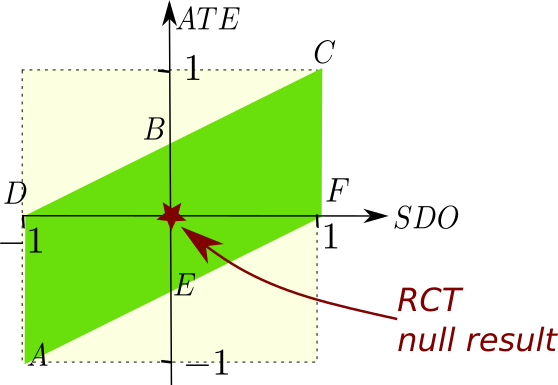
\includegraphics[width=2.5in]
{pot-out/sdo-ate-polytope.png}
\caption{
Green parallelogram
is accessible region in
$(SDO,ATE)$ plane,
assuming $y^\s\in \bool$.
Each of the
six points A, B, \ldots F
corresponds to one of the six tables
in Figs. \ref{fig-ate-possi}
and \ref{fig-sdo-possi}.
Segment $DF$
corresponds to the null
result in a RCT.
}
\label{fig-sdo-ate-polytope}
\end{figure}



\section{Matching Strata}

For a situation
described by
the bnet $G_{im+}$,
we can match {\it similar}
individuals to fill the blank cells of
 Table \ref{tab-pot-out-missing}.
By ``similar", we mean that
they have the same or almost the same
value of $\rvx^\s$.

IMPORTANT: Matching
only makes sense
if the individuals
are {\bf treatment blind} (i.e.,
have no knowledge
of whether they are
in the treated or control
groups.)


\subsection{Exact strata-match}

\subsubsection{Estimates of Treatment Effects}
\label{sec-estimates}
For $\td\in \bool$ and all strata $x$,
define the sets of individuals
$A_{\td,x}=\{\s: \td^\s=\td, x^\s=x\}$,
$A_x=A_{0,x}\cup A_{1,x}$ and $A=\cup_x A_x$.
Let $N_{\td,x}=|A_{\td,x}|$,
$N_x= |A_x|$ and $N=|A|$.

In an exact strata-match,
we match each individual with
$\td^\s=1, x^\s=x$
with
exactly
one individual
with $\td^\s=0, x^\s=x$
and vice versa.
Define a map $a:A\rarrow A$
such that,
for each $x$,
$m(A_{0,x})\subset A_{1,x}$ and
$m(A_{1,x})\subset A_{0,x}$.
This assumes $A_{0,x}$ and $A_{1,x}$
are non-empty for all $x$.
The purpose of map $m()$
is
to fill in the missing data in the
PO dataset. See Fig.\ref{tab-po-s-map}
for a pictorial representation of
this.

\begin{table}[h!]
\centering
\begin{tabular}{|l|l|l|}
\hline
 & \cellcolor[HTML]{ECF4FF}$y^\s(0)$ & \cellcolor[HTML]{ECF4FF}$y^\s(1)$ \\ \hline
\cellcolor[HTML]{ECF4FF}$\td^\s=0$ & $y^\s$ & $y^{m(\s)}$ \\ \hline
\cellcolor[HTML]{ECF4FF}$\td^\s=1$ & $y^{m(\s)}$ & $y^\s$ \\ \hline
\end{tabular}
\caption{Illustration of the
purpose of the map $m()$.
Note that $y^\s=y^\s(\td^\s)$ and $y^{m(\s)}=y^\s(!\td^\s)$,
where $!0=1$ and $!1=0$.}
\label{tab-po-s-map}
\end{table}


Note that

\beq
E_x[\rvtd^\s \rvy^\s]\neq
E_x[\rvtd^\s]\;\;E_x[ \rvy^\s]
\eeq
but
\beq
E_x[\rvd^\s \rvy^\s]=
E_x[\rvd^\s]\;\;E_x[ \rvy^\s]
\eeq
because, by d-separation, at fixed $x$,
 $\rvy^\s$ and $\rvtd^\s$
are not independent
but $\rvy^\s$ and $\rvd^\s$ are.

Note that
\beq
\sum_{\s\in A_{x}}\frac{\td^\s}{N_{1,x}}=
\sum_{\s\in A_{1,x}}\frac{1}{N_{1,x}}=1
\;.
\eeq
Thus

\beq
\sum_{\s\in A_{x}}\frac{\td^\s}{N_{1,x}}y^\s=
E_{\s|\td=1,x}[y^\s(1)]=\caly_{1|1,x}
\eeq
Table \ref{tab-po-quadrants}
gives
estimates of
$ \caly_{c|\td ,x}$

{\renewcommand{\arraystretch}{1.5}
\begin{table}[h!]
\centering
\begin{tabular}{|l|l|l|}
\hline
 & \cellcolor[HTML]{ECF4FF}$y^\s(0)$
& \cellcolor[HTML]{ECF4FF}$y^\s(1)$
\\ \hline
\cellcolor[HTML]{ECF4FF}$\td^\s=0$
&
$\frac{1}{N_{0,x}}\sum_{\s\in A_x} (1-\td^\s)y^{\s}=\caly_{0|0,x}$
&
$\frac{1}{N_{0,x}}\sum_{\s\in A_x} (1-\td^\s) y^{m(\s)}=\caly_{1|0,x}$
\\ \hline
\cellcolor[HTML]{ECF4FF}$\td^\s=1$
&
 $\frac{1}{N_{1,x}}\sum_{\s\in A_x} \td^\s y^{m(\s)}=\caly_{0|1,x}$
&
$\frac{1}{N_{1,x}}\sum_{\s\in A_x} \td^\s y^\s=\caly_{1|1,x}$
\\ \hline
\end{tabular}
\caption{Estimates of
$ \caly_{c|\td ,x}$.}
\label{tab-po-quadrants}
\end{table}
}


Recall that

\begin{subequations}
\label{eq-to-estimate}



\beq
ATE_x = ATT_x \;\;P_{\rvd|\rvx}(1|x) + ATU_x \;\;P_{\rvd|\rvx}(0|x)
\eeq

\beq
ATT_x=
\caly_{1|1,x}-\caly_{0|1,x}
\eeq

\beq
ATU_x=
\caly_{1|0,x}-\caly_{0|0,x}
\eeq

\beq
SB_x=\caly_{0|1,x}-\caly_{0|0,x}
\eeq


\beq
SDO_x=\caly_{1|1,x}-\caly_{0|0,x}
\eeq


\end{subequations}

Eqs.(\ref{eq-to-estimate})
can be estimated from the data
via the following estimators.



\beqa
\widehat{ATE}_x
&=&
\frac{1}{N_x}[
\widehat{ATT}_x N_{1,x} +
\widehat{ATU}_x N_{0,x}]
\\
&=&
\frac{1}{N_x}
\left[\sum_{\s\in A_x} \td^\s [y^\s - y^{m(\s)}]+
\sum_{\s\in A_x}(1-\td^\s) [ y^{m(\s)}-y^\s]
\right]
\\
&=&
\frac{1}{N_x}\sum_{\s\in A_x} (2\td^\s-1)[y^\s -y^{m(\s)}]
\label{eq-est-ate}
\eeqa

\beqa
\widehat{ATT}_x
&=&
\overbrace{\frac{1}{N_{1,x}}\sum_{\s\in A_x} \td^\s y^\s}^{\caly_{1|1,x}}
 -
\overbrace{\frac{1}{N_{1,x}}\sum_{\s\in A_x} \td^\s y^{m(\s)}}^{\caly_{0|1,x}}
\\
&=&
\frac{1}{N_{1,x}}\sum_{\s\in A_x} \td^\s [y^\s - y^{m(\s)}]
\label{eq-est-att}
\eeqa


\beqa
\widehat{ATU}_x
&=&
\overbrace{\frac{1}{N_{0,x}}\sum_{\s\in A_x} (1-\td^\s) y^{m(\s)} }^{\caly_{1|0,x}}
 -
\overbrace{\frac{1}{N_{0,x}}\sum_{\s\in A_x} (1-\td^\s)y^\s}^{\caly_{0|0,x}}
\\
&=&
\frac{1}{N_{0,x}}\sum_{\s\in A_x} (1-\td^\s) [ y^{m(\s)}-y^\s]
\label{eq-est-atu}
\eeqa

\beq
\widehat{SB}_x =
\overbrace{\frac{1}{N_{1,x}}\sum_{\s\in A_x} \td^\s y^{m(\s)}}^{\caly_{0|1,x}}
-
\overbrace{\frac{1}{N_{0,x}}\sum_{\s\in A_x} (1-\td^\s)y^\s}^{\caly_{0|0,x}}
\label{eq-est-sb}
\eeq

\beq
\widehat{SDO}_x=
\overbrace{\frac{1}{N_{1,x}}\sum_{\s\in A_x} \td^\s y^\s}^
{\caly_{1|1,x}}
-
\overbrace{\frac{1}{N_{0,x}}\sum_{\s\in A_x} (1-\td^\s) y^\s}^
{\caly_{0|0,x}}
\label{eq-est-sdo}
\eeq

We've said before that strata
matching makes no sense
unless every individual
is treatment blind.
This means that
if the individuals are not
treatment blind,
the above estimators for
$ATE_x, ATT_x,ATU_x, SB_x$
are invalid because they depend on
$m()$. Only the estimator for $SDO_x$
is valid because it doesn't depend on $m()$.

Suppose we do linear regression
to fit a
hyperplane $y(x)$ to
the dataset set $\{(x^\s, y^\s):\s\}$,
and then we calculate
$\frac{d\rvy}{d\rvtd}=\delta$.
Out
of all
the treatment effects,
this $\delta$ is
probably (?) closest
to $ACE=ATE$.
Note also that the
linear regression
method
of estimating
$\delta$
does imputation
(guesses missing values)
by doing a linear fit.
One can also
use machine learning to
do a non-linear fit.
In contrast, the estimators
of treatment effects
presented in this section
do imputation by
non-linear matching.

\subsubsection{Example, estimation of treatment effects}


For $\s\in \{1,2, \ldots, 10\}$, define

\beq
m(\s)=
\left\{
\begin{array}{ll}
\s+5&\text{if }\s\leq 5
\\
\s-5&\text{if }\s >5
\end{array}
\right.
\eeq


{\renewcommand{\arraystretch}{1.5}
\begin{table}[h!]
\centering
\begin{tabular}{|l|l|l|l|l|l|l|}
\hline
\cellcolor[HTML]{ECF4FF} $\s$& \cellcolor[HTML]{ECF4FF}$\td^\s$ & \cellcolor[HTML]{ECF4FF}$y^\s$ & \cellcolor[HTML]{ECF4FF}$\td^\s y^\s$ & \cellcolor[HTML]{ECF4FF}$(1-\td^\s)y^\s$ & \cellcolor[HTML]{ECF4FF}$\td^\s y^{m(\s)}$ & \cellcolor[HTML]{ECF4FF}$(1-\td^\s)y^{m(\s)}$ \\ \hline
\cellcolor[HTML]{ECF4FF}1 & \cellcolor[HTML]{FFFFC7}0 & 0 & \cellcolor[HTML]{FFFFC7}0 & 0 & \cellcolor[HTML]{FFFFC7}0 & 0 \\ \hline
\cellcolor[HTML]{ECF4FF}2 & \cellcolor[HTML]{FFFFC7}0 & 0 & \cellcolor[HTML]{FFFFC7}0 & 0 & \cellcolor[HTML]{FFFFC7}0 & 1 \\ \hline
\cellcolor[HTML]{ECF4FF}3 & \cellcolor[HTML]{FFFFC7}0 & 1 & \cellcolor[HTML]{FFFFC7}0 & 1 & \cellcolor[HTML]{FFFFC7}0 & 1 \\ \hline
\cellcolor[HTML]{ECF4FF}4 & \cellcolor[HTML]{FFFFC7}0 & 1 & \cellcolor[HTML]{FFFFC7}0 & 1 & \cellcolor[HTML]{FFFFC7}0 & 1 \\ \hline
\cellcolor[HTML]{ECF4FF}5 & \cellcolor[HTML]{FFFFC7}0 & 1 & \cellcolor[HTML]{FFFFC7}0 & 1 & \cellcolor[HTML]{FFFFC7}0 & 1 \\ \hline
\cellcolor[HTML]{ECF4FF}6 & 1 & 0 & 0 & \cellcolor[HTML]{FFFFC7}0 & 0 & \cellcolor[HTML]{FFFFC7}0 \\ \hline
\cellcolor[HTML]{ECF4FF}7 & 1 & 1 & 1 & \cellcolor[HTML]{FFFFC7}0 & 0 & \cellcolor[HTML]{FFFFC7}0 \\ \hline
\cellcolor[HTML]{ECF4FF}8 & 1 & 1 & 1 & \cellcolor[HTML]{FFFFC7}0 & 1 & \cellcolor[HTML]{FFFFC7}0 \\ \hline
\cellcolor[HTML]{ECF4FF}9 & 1 & 1 & 1 & \cellcolor[HTML]{FFFFC7}0 & 1 & \cellcolor[HTML]{FFFFC7}0 \\ \hline
\cellcolor[HTML]{ECF4FF}10 & 1 & 1 & 1 & \cellcolor[HTML]{FFFFC7}0 & 1 & \cellcolor[HTML]{FFFFC7}0 \\ \hline
\end{tabular}
\caption{Estimators of treatment effects
are calculated for this example. }
\label{tab-po-example}
\end{table}
}


\begin{table}[h!]
\centering
\begin{tabular}{|
>{\columncolor[HTML]{ECF4FF}}l |l|l|}
\hline
\cellcolor[HTML]{CBCEFB}$N(\td, y)$ & \cellcolor[HTML]{ECF4FF}$y=0$ & \cellcolor[HTML]{ECF4FF}$y=1$ \\ \hline
$\td=0$ & 2 & 3 \\ \hline
$\td=1$ & 1 & 4 \\ \hline
\end{tabular}
\caption{$N(\ul{\td^\s}=d, \rvy^\s=y)$ for
the data in Table \ref{tab-po-example}.}
\label{tab-n-po-example}
\end{table}

Let $N(\cals)$
be the number of individuals $\s$
that satisfy condition $\cals$.
For example,
$N(\ul{\td^\s}=\td)$
is the number of individuals
such that $\ul{\td^\s}=\td$.

\beq
N_1
=
N(\td^\s=1)
=
5
\eeq

\beq
N_0
=
N(\td^\s=0)
=
5
\eeq

\beq
N
= N_0+N_1
=
10
\eeq



\beq
\caly_{1|1}
=
\frac{1}{N_1}
\sum_\s \td^\s y^\s
=
\frac{4}{5}
\eeq

\beq
\caly_{0|0}
=
\frac{1}{N_0}
\sum_\s (1-\td^\s) y^\s
=
\frac{3}{5}
\eeq

\beq
\caly_{0|1}
=
\frac{1}{N_1}
\sum_\s \td^\s y^{m(\s)}
=
\frac{3}{5}
\eeq

\beq
\caly_{1|0}
=
\frac{1}{N_0}
\sum_\s (1-\td^\s) y^{m(\s)}
=
\frac{4}{5}
\eeq

\beq
ATT=
\caly_{1|1}-\caly_{0|1}
=\frac{1}{5}
\eeq

\beq
ATE=ATT=ATU=SDO=\frac{1}{5}
\;,\;\; SB=0
\label{eq-all-equal}
\eeq

This example is unusual
in that it has a single
stratum $x$, and for
that stratum,
the treated and
untreated populations
are {\bf balanced} (of equal size).
Also, the map $m()$
is 1-1 onto.
If, for instance,
$m(\s)=6$ for all $\s\in A_0$
and $m(\s)=5$ for $\s\in A_1$,
then $ATE, ATT, ATU, SDO$
would not all be same, and
$SB$ would not be zero.
In fact, whenever there is a single
balanced stratum and the map $m()$
is 1-1 onto, Eq.(\ref{eq-all-equal})
can be proven to be true using
the methods of
section \ref{sec-td-ignored}.



\subsection{Approximate strata-match}

It is very often
the case that
one can't
find for a given
individual $\s$
another individual that has
opposite $\td^\s$ but
exactly the same value of $x^\s$.
In such cases, one can discard all
matchless individuals.
But that would entail a loss
of precious information.
Instead of discarding orphans,
a better way is to
relax our demands and
match individual $\s$
with another individual $m(\s)$
such that $x^\s$
and $x^{m(\s)}$ are very
close in some metric.
Alternatively, the matching
individual might
not be real; it might
be a composite
of individuals.

More precisely,
for some arbitrary
parameter $\eps>0$,
and an individual $\s$
with $\td^\s=1$,
define
the {\bf strata-matching set}
$\calm_{\eps}(\s)$ by\footnote{
One can use an $\eps$
that depends on $\s$.
Let $\eps(\s, 5)$
be the radius necessary
so that $\calm_{\eps(\s, 5)}(\s)$
contains exactly 5 elements $m$.
Thus, $\calm_{\eps(\s, 5)}(\s)$
contains the $m$ of the
 5 points $x^m$ that are the
nearest neighbors of $x^\s$
in the $dist()$ metric.}

\beq
\calm_{\eps}(\s)=
\{m: \td^\s=1, \td^m=0,
dist(x^\s, x^m)\leq \eps \}
\;,
\eeq
where

\beq
dist(x^\s, x^m)=
[x^\s]^T [\Sigma]^{-1} x^m
\;,
\eeq
where $\Sigma = \av{\rvx^\s, [\rvx^m]^T}$.
 This
metric $dist(x^\s, x^m)$ is
called the {\bf Mahalanobis distance}.
We will call
the case $\eps=0$ an {\bf  exact strata-match},
and
the case
$\eps\neq 0$
 an {\bf approximate strata-match.}.
To do an approximate strata-match,
replace $y^{m(\s)}$
by
$\av{y}^\s$
in
the estimators
given above
for an exact strata-match.
$\av{y}^\s$
is defined by

\beq
\av{y}^\s=
\frac{1}{|\calm_{\eps}(\s)|}
\sum_{m\in \calm_{\eps}(\s)}
y^m
\;.
\eeq

Ref.\cite{book-mixtape}
calculates the mean and variance
of estimator $\widehat{ATT}_x$.
The mean is biased,
but one can define a new
bias-corrected estimator.


\section{Positivity}


{\bf Positivity} is defined as the
requirement that for all layers $x$,
\beq
0<P(\rvd^\s=1|\rvx^\s=x)<1
\eeq
or, equivalently,
\beq
P(\rvd^\s=1|\rvx^\s=x)>0\text{\;\;\;and
\;\;\;}P(\rvd^\s=0|\rvx^\s=x)>0
\;.
\eeq
In other words,
for each layer $x$,
there is
a non-zero
probability of being both treated
and untreated.

Recall that

\beq
\caly_{c|\td ,x}
=\sum_{y} y P_{\rvy(c)|\rvtd, \rvx}(y|\td,x)
\;.
\eeq
Also recall
that the estimator
Eq.(\ref{eq-est-att})
for $ATT_x$ divides by $N_{1,x}=P(\rvd=1|x)N_x$
and
the estimator
Eq.(\ref{eq-est-atu})
for $ATU_x$ divides by $N_{0,x}= P(\rvd=0|x)N_x$.
The estimator Eq.(\ref{eq-est-ate})
for $ATE_x$ divides by neither $N_{0,x}$
nor $N_{1,x}$ so it is safe.

If positivity is violated,
then
for some
layer $x$,
 $\caly_{c|\td =0,x}$ or $\caly_{c|\td =1,x}$
is undefined.
Furthermore,  the estimator
$ATT_x$ or $ATU_x$ is undefined.
If $ATT_x$ (or any
other treatment effect)  can be estimated,
one says it is {\bf do-identifiable} (i.e.,
expressible without do() operators).
If Positivity is violated, then
either $ATT_x$ or $ATU_x$ is not identifiable.



When
$P(d^\s|x^\s=x)$
becomes 0 or 1 for some $x$,
the arrow
$\rvx\rarrow\rvd$
becomes deterministic
for some $x$.
This situation
is
the very
antithesis
of RCTs,
wherein
the influence
exerted by $\rvx^\s$ on
$\rvd^\s$ is uniformly
random and therefore ignorable.
Hence, it is perhaps
not too surprising
that a violation
of positivity makes
$ATT$ or $ATU$
not identifiable.

\section{Propensity Score
Weighting}

Let

\beq
g_d(x)=P_{\rvd|\rvx}(d|x)
\eeq
 for $d\in\bool$.
Note that $g_0(x)+g_1(x)=1$.
$g_1(x)$ is called the {\bf propensity score}.
One can do {\bf propensity score weighting}
within the estimators
presented in Section
\ref{sec-estimates} to
improve their behavior.
This is done by making the
following replacements.

\beq
N_{1,x}
\rarrow
N_x g_1(x^\s)
\;,\;\;
N_{0,x}
\rarrow
N_x g_0(x^\s)
\;.
\eeq
These replacements are
equal under $ \sum_{\s\in A_x}$
to the terms they replace.

\begin{claim}
\label{cl-d-line}
Suppose $g_0+g_1=1$ and

\beq F(d)=
\frac{d}{g_1}-\frac{(1-d)}{g_0}
\;.
\eeq
Then
\beq
F(d)=
\frac{d-g_1}{g_0g_1}
\;.
\eeq
\end{claim}
\proof
You can do the algebra
or simply check mentally that
$F(0)=\frac{-1}{g_0}$
and $F(1)=\frac{1}{g_1}$
for both versions of $F()$.
\qed

As an example of
Propensity Score Weighting, note that

\begin{claim}

\beq
\widehat{SDO}_x=
\frac{1}{N_x}
\sum_{\s\in A_x}
\frac{y^\s[\td^\s-g_1(x^\s)]}
{g_1(x^\s)[1-g_1(x^\s)]}
\label{eq-est-sdo-fancy}
\eeq
\end{claim}
\proof
\beqa
\widehat{SDO}_x&=&
\frac{1}{N_x}
\sum_{\s\in A_x}
y^\s
\left[
\frac{\td^\s}{g_1(x^\s)}
-
\frac{(1-\td^\s)}{g_0(x^\s)}
\right]\;\;
\text{(from Eq.(\ref{eq-est-sdo}))}
\label{eq-sum-sdo-psw-div}
\\
&=&
\frac{1}{N_x}
\sum_{\s\in A_x}
y^\s
\left[
\frac{\td^\s -g_1}
{g_0 g_1}
\right]\;\;\text{(by Claim \ref{cl-d-line}.)}
\eeqa
\qed

I've seen
some texts claim that
Eq.(\ref{eq-est-sdo-fancy})
is an estimate of $ATE_x$.
I don't think so.
As we saw when exploring the $(SDO,ATE)$
space, $SDO$ and $ATE$
can be quite different.
Lots of admissible points
fall outside the $ATE=SDO$ line.

Dividing
each term
in the sum Eq.(\ref{eq-sum-sdo-psw-div})
by $g_\td(x)$ has the following effect.
$g_\td(x)=P(\rvd=\td|x)$ is the
likelihood of strata $x$,
so dividing each term by
this likelihood increases the
contribution to the sum
by less likely strata
and decreases the contribution by
more likely strata.


You may have noticed that
we used
\begin{subequations}
\beq
N_{\td,x}=N_x g_\td(x)=N_x P({\color{red}\rvd}=\td|x)
\label{eq-incorrect-psw}
\eeq
above.
Why didn't we use
\beq
N_{\td,x}=N_x P({\color{red}\rvtd}=\td|x)=N_x P({\color{red}\rvtd}=\td)
\label{eq-correct-psw}
\eeq
\end{subequations}
 instead?
I think that
Eq.(\ref{eq-correct-psw})
is correct
and
Eq.(\ref{eq-incorrect-psw})
is incorrect,
but the latter
is a reasonable approximation
of the former, because recall that
we usually define

\beq
P(\rvtd=\td)=\sum_x P(\rvd=\td|x)P(x)
\;.
\eeq
The incorrect Eq.(\ref{eq-incorrect-psw})
is basically assuming that nodes
$\rvd$ and $\rvtd$ are the same node (imagine $G_{im}$
in Fig.\ref{fig-po-G-im-y0-y1}
with nodes $\rvd$ and $\rvtd$ merged). This
is
a common mistake in PO theory texts.
But if we merge those two nodes,
CIA no longer holds.



\section{Propensity Score}

It is often the case
that the discrete vector $\rvx^\s$
has
too many possible values to make
matching possible.
In such cases, it
is convenient to
map the space
of vectors
$\rvx^\s$
to the real line.
One very
convenient choice
for that map
is the
{\bf propensity score},
which is defined as

\beq
g(x^\s)=P(\rvd^\s=1|x^\s)
\;.
\eeq
$P(\rvd^\s=1|x^\s)$ is easy to calculate
from the dataset.
Indeed,
if $\Sigma_{d,x}=
\{\s\in\Sigma: d^\s=d, x^\s=x\}$ and
$N_{d, x}=|\Sigma_{d,x}|$,
then

\beq
P(\rvd=1|x^\s=x)=
\frac{N_{d=1,x}}{\sum_{d\in\bool} N_{d,x}}
\;.
\eeq


\begin{figure}[h!]
$$
\xymatrix{
\rvg^\s\ar[d]
&\rvx^\s\ar[dr]\ar[l]
\\
\rvd^\s&\rvtd^\s\ar[r]&\rvy^\s
\\
&G_{ps}
}
$$
\caption{Bnet $G_{ps}$
used when doing propensity scoring.}
\label{fig-po-G-ps}
\end{figure}
To use the
propensity score,
one replaces the bnet $G_{im+}$
by the bnet $G_{ps}$
shown in Fig.\ref{fig-po-G-ps}.
The TPMs, printed in blue,
for the 2 nodes of $G_{ps}$
that differ from the nodes
of $G_{im+}$,
are as follows:


\beq\color{blue}
P(g^\s|x^\s)=
\delta(g^\s, g(x^\s))
\eeq

\beq\color{blue}
P(d^\s|g^\s)=
g^\s d^\s + (1-g^\s)(1-d^\s)
\eeq

Note that
these TPMs are self-consistent because

\beqa
P(d|x)&=&
\sum_g P(d|g)P(g|x)
\\
&=&
g(x)d + [1-g(x)](1-d)
\\
&=&
P(\rvd=1|x)d + [1-P(\rvd=1|x)](1-d)
\\
&=&
P(d|x)
\eeqa


We would like to do
{\bf propensity score strata-matching} by
matching g-strata instead of x-strata.
 PO calculations
for x-strata matching
use the TPMs
for $P(d|x)$, $P(x)$
and $P(y|d,x)$.
To do g-strata matching
using the same
equations, but
with $x$ replaced by $g$,
we would need to solve for
$P(d|g)$, $P(g)$
and $P(y|d,g)$
in terms of
$P(d|x)$, $P(x)$
and $P(y|d,x)$.
We solve for those next.

From the TPMs
for $G_{ps}$, one has

\beq
\boxed{
P(d|g)=
g d + (1-g)(1-d)}
\eeq
and

\beq
\boxed{
P(g)=\sum_x \overbrace{
\delta(g,g(x))}^{P(g|x)}
P(x)}
\;.
\eeq
Next, note that


\beq
P(y| d,g)=
\sum_x P(y|d,x)P(x|g)
\eeq
so we need to find $P(x|g)$. Since

\beqa
P(x|g)&=&\frac{P(g|x)P(x)}{P(g)}
\\
&=&
\frac{\delta(g, g(x))P(x)}{P(g)}
\eeqa
we finally get

\beq
\boxed{
P(y| d,g)=
\sum_x P(y|d,x)
\frac{\delta(g, g(x))P(x)}{P(g)}
}
\;.
\label{eq-p-y-dg}
\eeq

Eq.(\ref{eq-p-y-dg})
looks complicated, but all
it is saying is that, given
any function $\calf(g)$ of $g$,

\beq
\sum_g P(g)\calf(g) P(y|d,g)=
\sum_x P(x)\calf(g(x)) P(y|d,x)
\;.
\eeq



\section{Multi-time PO bnets (Panel Data)}

In this section, we will
discuss Multi-time PO bnets (MT-PO).

A {\bf time-series} is a function $f:D\rarrow \RR$
whose domain $D$ is a discrete set
of times. A time-series
usually describes a single
unit $\s$ (i.e., an individual)
in a population.

An {\bf observational study (or analysis or model)}
can be cross-sectional or longitudinal.
A {\bf cross-sectional study}
collects and analyzes a {\bf cross-sectional dataset};
i.e., a dataset for a population
at a single time. A {\bf longitudinal study
or panel study} collects and analyzes
a {\bf longitudinal dataset};
i.e., a dataset for a population
at  multiple times.
Thus, a longitudinal study
consists of one or more time-series.

Let $\calt=\{t_0, t_1, \ldots, t_{ntimes-1}\}$.
For any time-series $a_t: \calt\rarrow\RR$,
define

\beq
E_t a_t=
\frac{1}{ntimes}\sum_{t\in \calt} a_t
\eeq

\beq
\Delta_t a_t = a_t -E_t a_t
\eeq

\beq
\av{a_t, b_t}_t= E_t \Delta_t a_t \Delta_t b_t
\eeq

Consider a quantity $a^\s_t$
that is a function of  the time $t$
and of the particular unit $\s$
in a population.
$a^\s_t$ is said to be a {\bf fixed (in time) effect}
if it is $t$-independent.
$a^\s_t$ is said to be a
{\bf homogeneous effect}
(antonym: {\bf heterogeneous effect})
if it is
$\s$-independent.
Henceforth, we will avoid
using the word ``effect" for these
because that word
 has already been used for something else in
PO theory.
Instead, we will use the word ``quantity".

\begin{figure}[h!]
$$\xymatrix @C=4pc {
\rvu^\s\ar@/^1pc/@{-->}[dd]\ar@/^2pc/@{-->}[ddd]
&\rvu^\s\ar@/^1pc/@{-->}[dd]\ar@/^2pc/@{-->}[ddd]
&\rvu^\s\ar@/^1pc/@{-->}[dd]\ar@/^2pc/@{-->}[ddd]
\\
\rvx^\s\ar[d]_\gamma\ar@/_1.5pc/[dd]_\beta
&\rvx^\s\ar[d]\ar@/_1.5pc/[dd]
&\rvx^\s\ar[d]\ar@/_1.5pc/[dd]
\\
\rvd^\s_0\ar[d]_\delta\ar[r]_\alp
&\rvd^\s_1\ar[d]\ar[r]
&\rvd^\s_2\ar[d]
\\
\rvy^\s_0
&\rvy^\s_1
&\rvy^\s_2
}$$
\caption{Example
of multi-time PO bnet
with fixed quantities $\rvx^\s, \rvu^\s$.
The
3 nodes $\rvx^\s$
should be identified
as a single node.
 Likewise, the
3 nodes $\rvu^\s$
should be identified
as a single node.
}
\label{fig-dynamic-po}
\end{figure}

Fig.\ref{fig-dynamic-po}
gives an example
of a multi-time PO bnet (MT-PO).
Note that in this example, $\rvx^\s$
and $\rvu^\s$ are fixed quantities (i.e.,
 they are $t-$independent).
$\rvu^\s$ is an unobserved confounder
and $\rvx^\s$ is an observed confounder.
For convenience and simplicity, we will assume linear
deterministic TPMs  for
the internal (i.e., non-root)  nodes.
The TPMs for the bnet Fig.\ref{fig-dynamic-po},
printed in blue, are as follows:

\beq\color{blue}
P(x^\s)=P_\rvx(x^\s)
\eeq

\beq\color{blue}
P(u^\s)=P_\rvu(u^\s)
\eeq

\beq\color{blue}
P(y^\s_t|d^\s_t,x^\s, u^\s)=\indi(\;\;
y^\s_t=
\delta d^\s_t + \beta x^\s  +u^\s\;\;)
\eeq

\beq\color{blue}
P(d^\s_{t+1}|d^\s_t, x^\s, u^\s)=\indi(\;\;
d^\s_{t+1}=  \alp d^\s_t + \gamma x^\s+ u^\s\;\;)
\eeq

Taking time averages
of the treatment dose and
treatment outcome, we get


\beq
E_t \rvy^\s_t=
\delta E_t \rvd^\s_t + \beta \rvx^\s  +\rvu^\s
\;,
\eeq

\beq
E_t \rvd^\s_{t+1}=  \alp E_t \rvd^\s_t +
 \gamma \rvx^\s+ \rvu^\s
\;.
\eeq
Subtracting the time averages from the
quantities being averaged, we get


\beq
\Delta_t \rvy^\s_t=
\delta\Delta_t  \rvd^\s_t
\;,
\eeq

\beq
\Delta_t \rvd^\s_{t+1}=  \alp \Delta_t \rvd^\s_t
\;.
\eeq
This allows us to find estimators for $\delta$
and $\alp$:



\beq
E_\s\av{\rvy^\s_t, \rvy^\s_t}_t
=\delta E_\s\av{\rvy^\s_t, \rvd^\s_t}_t
\eeq

\beq
\delta=
\frac{E_\s\av{\rvy^\s_t, \rvy^\s_t}_t
}{
E_\s\av{\rvy^\s_t, \rvd^\s_t}_t
}
\eeq

\beq
E_\s\av{\rvd^\s_{t+1}, \rvd^\s_{t+1}}_t
=\alp E_\s\av{\rvd^\s_{t+1}, \rvd^\s_t}_t
\eeq

\beq
\alp=
\frac{E_\s\av{\rvd^\s_{t+1}, \rvd^\s_{t+1}}_t
}{
E_\s\av{\rvd^\s_{t+1}, \rvd^\s_t}_t
}
\eeq

As shown in Fig.\ref{fig-dynamic-po-avg},
 subtraction
of time averages
from each node removes the
confounder nodes from the bnet
of Fig.\ref{fig-dynamic-po} (However, this
assumes that the
confounders are time independent
and that the TPMs
for the internal nodes
are linear deterministic,
two very strong assumptions).

\begin{figure}[h!]
$$\xymatrix @C=4pc {
\Delta_t\rvd^\s_{t}\ar[d]_\delta\ar[r]_\alp
&\Delta_t\rvd^\s_{t+1}\ar[d]
\\
\Delta_t\rvy^\s_t
&\Delta_t\rvy^\s_{t+1}
}$$
\caption{time-average-subtracted (TAS) bnet for the bnet
of Fig.\ref{fig-dynamic-po}.
}
\label{fig-dynamic-po-avg}
\end{figure}